\section{Semantic LSP}%
\label{sec:semantic_lsp}

When developing a LSP, we made sure to follow the state of the art best implementation practices\cite{10.1145/3550355.3552452,10.1145/3563834.3567537,10.1145/3550355.3552452,Bour_2018}.
Semantic LSP is built on top of an entity component system, allowing for even greater seperation of concern than the proposed \textit{Layered Architecture}\cite{10.1145/3550355.3552452}.

Entity component system is a software pattern that involves breaking your program up into Entities, Components, and Systems.
Entities are unique "things", here documents, that are assigned groups of Components, which are then processed using Systems.
Components include the contents of the source file, the location of the source file, the derived triples, etc.
Systems are functions that are grouped in schedules, one system might derive defined owl properties from derived triples and might be present in the \textit{Parse} schedule.
Each language can then add their specific systems into the defined schedules for language specific functionality.
This way common systems are defined once, resulting in a consistent experience over all semantic languages.
Bour et al. state "No spec, no tests"\cite{Bour_2018}, meaning it is difficult to write a useful testsuite for language servers.
User-facing features are not well specified and open for interpretation.
At least common systems act the same way over different semantic languages.

\subsection{Langauge Server schedules}

This section goes into detail on the different systems that are implemented for each schedule of the language server.
Some systems only create components, these components are then used by other systems, potentially in different schedules.
If an expected component is not present, the system will skip that entity, allowing for asynchronously running systems.

\subsubsection*{Parse}

The parsing schedule is one of the most important schedules of the language server.
It is activated whenever the user edits a document, the language server is notified with the textual changes.
With the language server protocol the server can specify wether or not it requires only the (minimal) changes or entire document every time.
Earlier versions of the semantic lsp required the entire document every time, because documents arae relatively small and reprasing the entire document brings an acceptable performance.
However, we noticed that this hampered the implementation, in turtle specifically there are patterns that cannot be parsed correctly and brings incorrect and frustrating feedback to the user, and partial parsing helps in this regard.
An example is shown in \ref{lst:GroupedListing}.
  The user at \ref{code1} types named node \texttt{<b>}, the language server should not be confused: triple \texttt{<c> <d> <e>} has nothing to do with named node \texttt{<b>}. The language server should suggest objects that fulfill the domain of predicate \texttt{<b>}. 
  The user at \ref{code2} types named node \texttt{<c>}, the language server should not be confused: the are two triples \texttt{<a> <b> <c>} and \texttt{<a> <d> <e>}, however tokenwise the documents are the same. Resulting in the language server suggesting a semi colon.
  
  The user at \ref{code3} just wrote a subject, invocing the subject completion defined in the next section. The language server might incorrect suggest to add a comma after \texttt{<c>} to build a syntactically correct document.
  The user at \ref{code4} is typing a predicate for the subject \texttt{<a>}, the language server might incorrectly parse the document as seen at \ref{code3}, where \texttt{<b>} is subject thus not invocing the property completion as explained in the next section.

  Adding partial parsing eliminates these issues as the language server understand which tokens are new and leaving the original interpretation of the surrounding tokens in touch.


\begin{figure}[htb]
    \centering
    % code1
    \begin{subfigure}{0.2\textwidth}
      \lstinputlisting{./code/option1.ttl}
      \caption{User types \texttt{<b>}}
      \label{code1}
    \end{subfigure}
    \hfill
    % code 2
    \begin{subfigure}{0.2\textwidth}
      \lstinputlisting{./code/option2.ttl}
      \caption{User types \texttt{<c>}}
      \label{code2}
    \end{subfigure}
    \hfill
    % code 3
    \begin{subfigure}{0.2\textwidth}
      \lstinputlisting{./code/option3.ttl}
      \caption{User types \texttt{<a>}}
      \label{code3}
    \end{subfigure}
    \hfill
    % code 4
    \begin{subfigure}{0.2\textwidth}
      \lstinputlisting{./code/option4.ttl}
      \caption{User types \texttt{<b>}}
      \label{code4}
    \end{subfigure}
    \caption{Grouped code listings for demonstration purposes.}\label{lst:GroupedListing}
\end{figure}


\begin{figure}[!ht]
 \centering
 \makebox[\textwidth]{%
    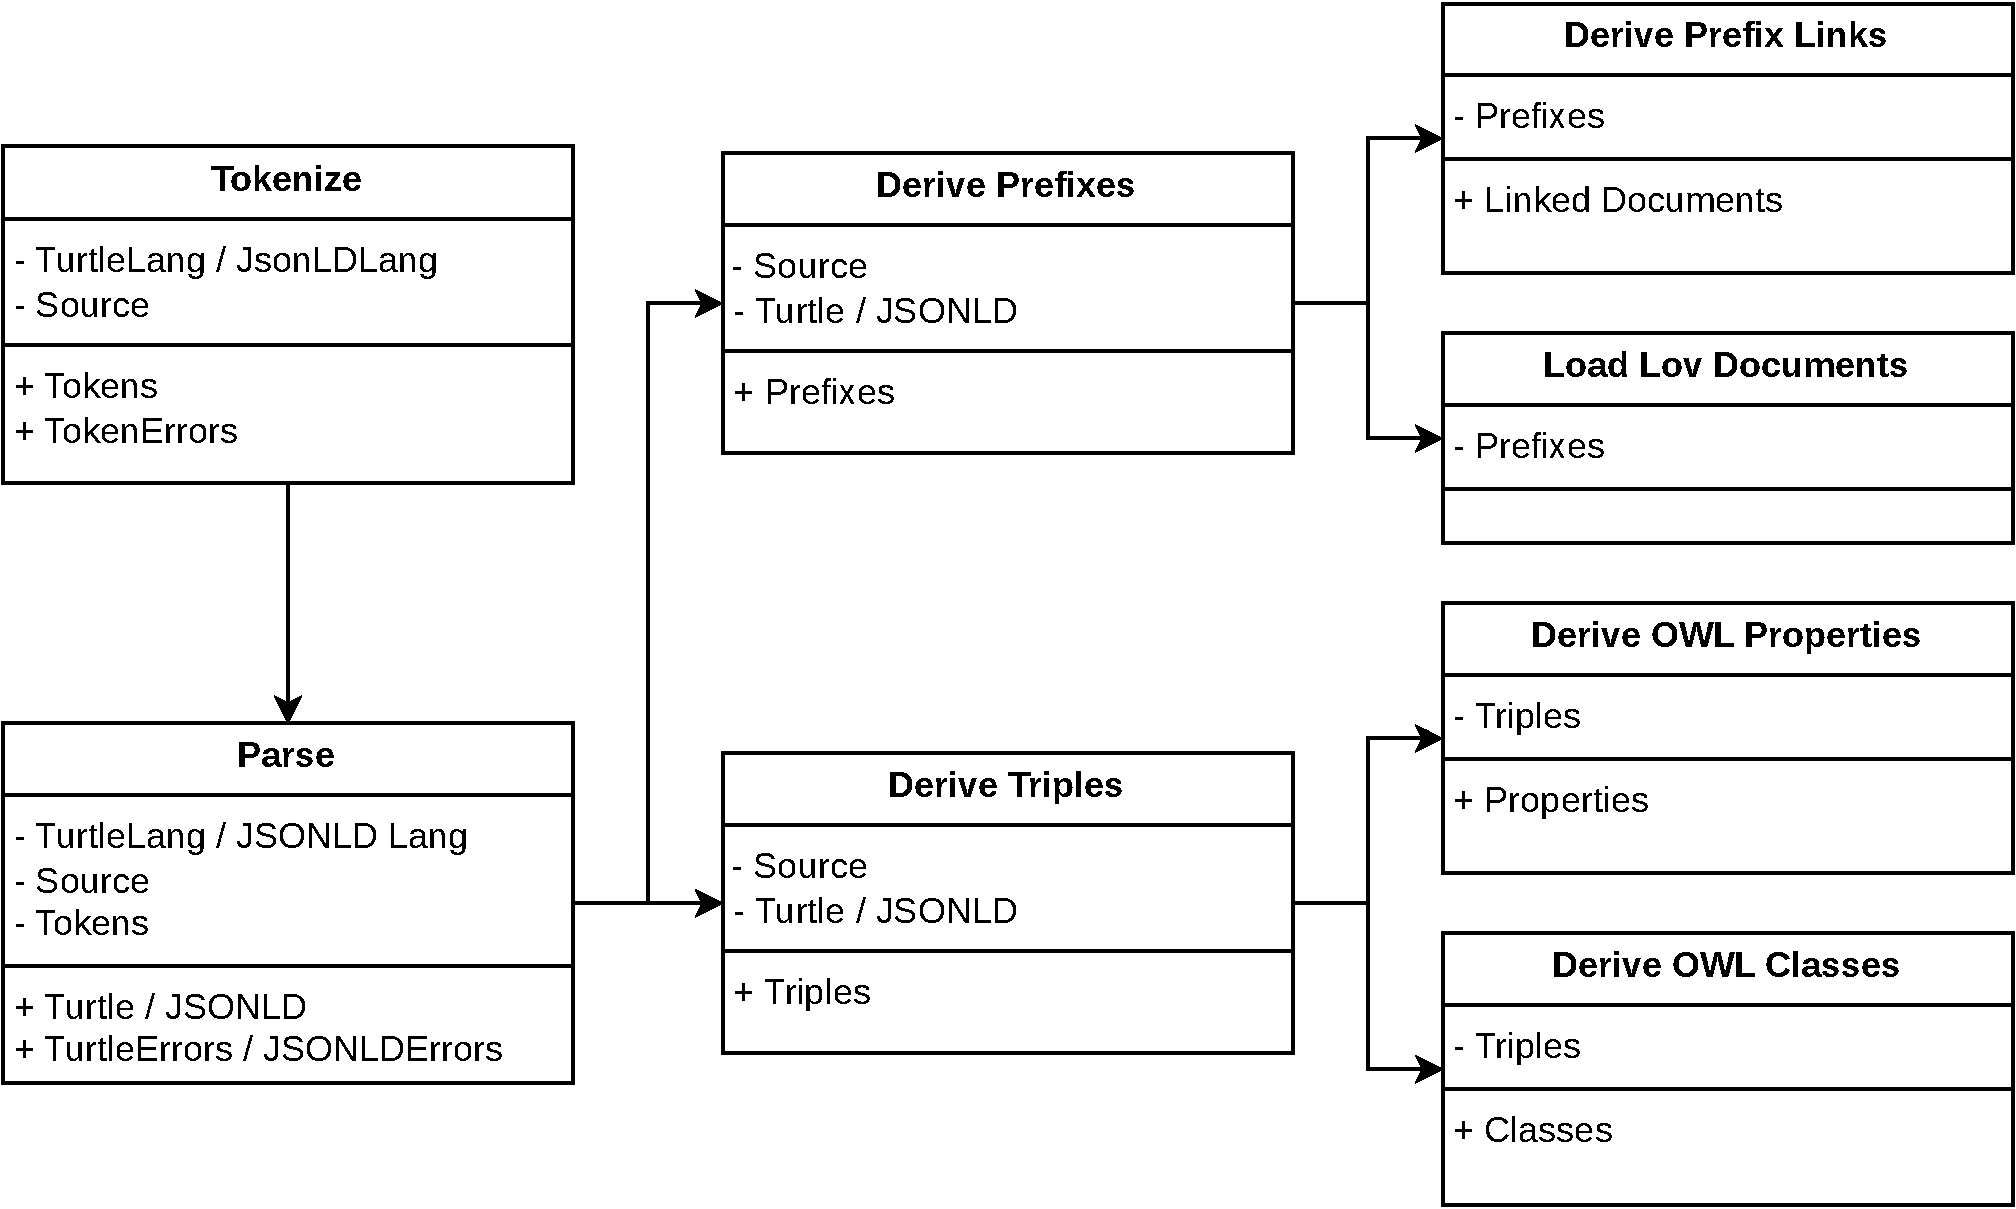
\includegraphics[width=1.2\textwidth]{./images/ParseSchedule.pdf}
 }
  \caption{Visual representation of our example pipeline, 
      loading sensor data from The Things Network into a triple store}\label{fig:Parse}
\end{figure}


\subsubsection*{Completion}


\begin{figure}[!ht]
 \centering
 \makebox[\textwidth]{%
    \includegraphics[width=1.2\textwidth]{./images/Completion.pdf}
 }
  \caption{Visual representation of our example pipeline, 
      loading sensor data from The Things Network into a triple store}\label{fig:Completion}
\end{figure}

\subsubsection*{Diagnostics}




\subsubsection*{SemanticHighlighting}

